\documentclass[tikz,border=8pt]{standalone}
\usepackage{tikz}
\usetikzlibrary{arrows.meta,calc,positioning}
\usepackage{xcolor}
\renewcommand{\familydefault}{\sfdefault}
\pagecolor{gray!12}

% -------------------------
% Parameters
% -------------------------
\newcommand{\NInput}{6}
\newcommand{\NEncoder}{4}
\newcommand{\NLatent}{2}
\newcommand{\NDecoder}{4}
\newcommand{\NOutput}{6}

\newcommand{\XInput}{0}
\newcommand{\XEncoder}{2.6}
\newcommand{\XMu}{5.0}
\newcommand{\XLogVar}{6.2}
\newcommand{\XZ}{7.65}
\newcommand{\XDecoder}{9.7}
\newcommand{\XOutput}{12.3}

\newcommand{\LayerSep}{1.05}
\newcommand{\NeuronSize}{7.8mm}
\newcommand{\CalloutGap}{2.2mm}

\colorlet{InputColor}{green!18!white}
\colorlet{DistColor}{orange!10!white}
\colorlet{SampleColor}{orange!18!white}
\colorlet{OutputColor}{blue!12!white}

% -------------------------
% Helpers
% -------------------------
\newcommand{\PlaceLayer}[4]{%
  % #1 prefix, #2 count, #3 x-position, #4 fill color
  \pgfmathsetmacro{\HalfSpan}{(#2-1)/2}
  \foreach \i in {1,...,#2}{%
    \pgfmathsetmacro{\y}{(\HalfSpan-(\i-1))*\LayerSep}
    \node[circle,draw=black,thin,minimum size=\NeuronSize,inner sep=0pt,fill=#4] (#1\i) at (#3,\y) {};
  }%
}

\newcommand{\ConnectLayers}[4]{%
  % #1 left prefix, #2 left count, #3 right prefix, #4 right count
  \foreach \i in {1,...,#2}{%
    \foreach \j in {1,...,#4}{%
      \draw[black,thin] (#1\i) -- (#3\j);
    }%
  }%
}

\begin{document}
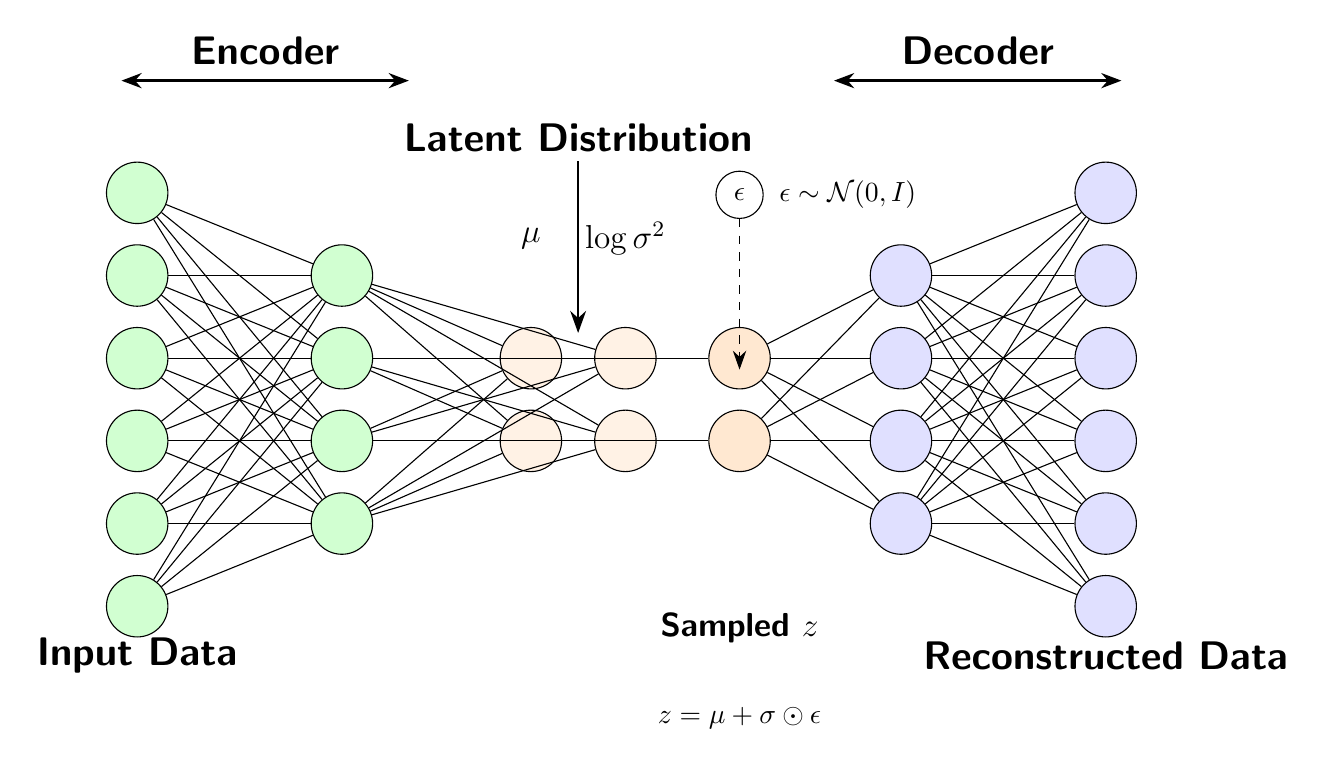
\begin{tikzpicture}[
  >=Stealth,
  title/.style={font=\sffamily\bfseries\Large},
  label/.style={font=\sffamily\bfseries\Large},
  smalllabel/.style={font=\sffamily\bfseries\large},
  note/.style={font=\sffamily\normalsize},
  callout/.style={line width=0.95pt,-{Stealth[length=2.8mm,width=2mm]}},
  noise/.style={circle,draw=black,thin,minimum size=6mm,inner sep=0pt,fill=white}
]

% Layers
\PlaceLayer{I}{\NInput}{\XInput}{InputColor}
\PlaceLayer{E}{\NEncoder}{\XEncoder}{InputColor}
\PlaceLayer{M}{\NLatent}{\XMu}{DistColor}
\PlaceLayer{V}{\NLatent}{\XLogVar}{DistColor}
\PlaceLayer{Z}{\NLatent}{\XZ}{SampleColor}
\PlaceLayer{D}{\NDecoder}{\XDecoder}{OutputColor}
\PlaceLayer{O}{\NOutput}{\XOutput}{OutputColor}

% Core network connections
\ConnectLayers{I}{\NInput}{E}{\NEncoder}
\ConnectLayers{E}{\NEncoder}{M}{\NLatent}
\ConnectLayers{E}{\NEncoder}{V}{\NLatent}
\ConnectLayers{Z}{\NLatent}{D}{\NDecoder}
\ConnectLayers{D}{\NDecoder}{O}{\NOutput}

% Reparameterization connections (paired for readability)
\foreach \i in {1,...,\NLatent}{%
  \draw[black,thin] (M\i) -- (Z\i);
  \draw[black,thin] (V\i) -- (Z\i);
}

% Noise source for the reparameterization trick
\node[noise] (eps) at ($(Z1)!0.5!(Z2)+(0.0,2.6)$) {$\epsilon$};
\draw[dashed,black,thin,-{Stealth[length=2.4mm,width=1.7mm]}] (eps.south) -- ($(Z1)!0.5!(Z2)+(0.0,0.38)$);
\node[note,anchor=west] at ($(eps)+(0.38,0.0)$) {$\epsilon \sim \mathcal{N}(0,I)$};

% Top arrows and section titles
\draw[<->,line width=0.95pt] (\XInput-0.2,4.05) -- node[above=2pt,title]{Encoder} (\XEncoder+0.85,4.05);
\draw[<->,line width=0.95pt] (\XDecoder-0.85,4.05) -- node[above=2pt,title]{Decoder} (\XOutput+0.2,4.05);

% Latent distribution title (centered over mu and logvar columns)
\node[title] (disttitle) at ($(M1)!0.5!(V1)+(0,2.8)$) {Latent Distribution};
\draw[callout] (disttitle.south) -- ($($(M1)!0.5!(V1)$)+(0,0.32)$);

% Small labels over the latent parameter heads and sampled latent
\node[smalllabel] at (\XMu,2.05) {$\mu$};
\node[smalllabel] at (\XLogVar,2.05) {$\log\sigma^2$};
\node[smalllabel] at (\XZ,-2.9) {Sampled $z$};

% Bottom labels
\node[label] at (\XInput,-3.25) {Input Data};
\node[label] at (\XOutput,-3.25) {Reconstructed Data};

% Reparameterization annotation
\node[note,align=center] at (\XZ,-4.05) {$z = \mu + \sigma \odot \epsilon$};

\end{tikzpicture}
\end{document}